% !TEX root = ../NeuralNetworksEN.tex

%%%%%%%%%%%%%%%%%%%%%%%%%%%%%%%%%%%%%%%%%%%%%%%%%%%%%%%%%%
%%%%%%%%%%%%%%%%%%%%%%%%%%%%%%%%%%%%%%%%%%%%%%%%%%%%%%%%%%
\section{Algorithmics and mathematics of learning}

Neural networks are algorithms, which compute, from an input $\myblue{x}$ (for example an image), an output ${\color{red} y}$. As shown in figure~\ref{fig:discriminative}, this output is most often a set of probabilities: for example the first output is the probability that the image contains a cat (the closer this number is to $100\%$, the more it means that the algorithm is sure of itself), the second is the probability that the image contains a dog, etc.
%
To simplify, we will consider in our examples only two classes: cats and dogs, but in practice one can consider an output ${\color{red} y}$ with several thousands of classes. We also restrict ourselves to the example of images, but neural networks are also very efficient in recognizing texts or videos.

Mathematically, such an algorithm defines a function $f_{\mygreen{w}}$ (i.e. ${\color{red} y} = f_{\mygreen{w}}({\color{blue}x})$). The computer program that calculates this function is very simple: it is made up of a sequence of several stages, and each stage performs elementary calculations (additions, multiplications, and a maximum).
%
In comparison, the computer programs found in a computer's operating system are much more complex.
%
But what makes the huge difference between a \guill{classical} algorithm and a neural network is that the latter depends on parameters, which are the weights of the neurons. Before using a neural network, these weights must be modified so that the algorithm can best solve the requested task. This is done using mathematical and algorithmic methods which will be explained in the following sections. This process is called \guill{training} a neural network, and this requires a lot of time, machine calculations and energy.

Using these algorithms wisely therefore requires computer science and mathematics skills. It is thus necessary to manipulate  key concepts in computer science (iterative methods, computation time, memory space, efficient implementation, \ldots) and mathematics (linear algebra, optimization, statistics, \ldots).

%%%%%%%%%%%%%%%%%%%%%%%%%%%%%%%%%%%%%%%%%%%%%%%%%%%%%%%%%%

\section{Discriminative neural networks}

An artificial neural network is built around a biological metaphor.
%
The structure of the primary visual cortex is relatively well known, and Hubel and Wiesel won the Nobel Prize in Physiology for the discovery in 1962 of the organization of neurons in the first cortical layers~\cite{hubel1962receptive}.
%
Thus, in an extremely simplified view of the brain, neurons are organized in layers, each neuron retrieves information from a previous layer, performs a very simple calculation, and communicates its result to neurons in the next layer.
%
It must however be keep in mind that this is only a metaphor and a source of inspiration: biological networks have much more complex connections and the mathematical equations which govern them are also more complex (they have been discovered by Alan Hodgkin and Andrew Huxley in 1952~\cite{hodgkin1952quantitative} and they won the Nobel Prize for this).
%
It therefore remains difficult to precisely relate the sometimes surprising performances of artificial neurons to the cognitive capacities of the brain. For example, the techniques to train artificial networks which I will now explain are quite different from the way a child learns.

\begin{figure}\centering
	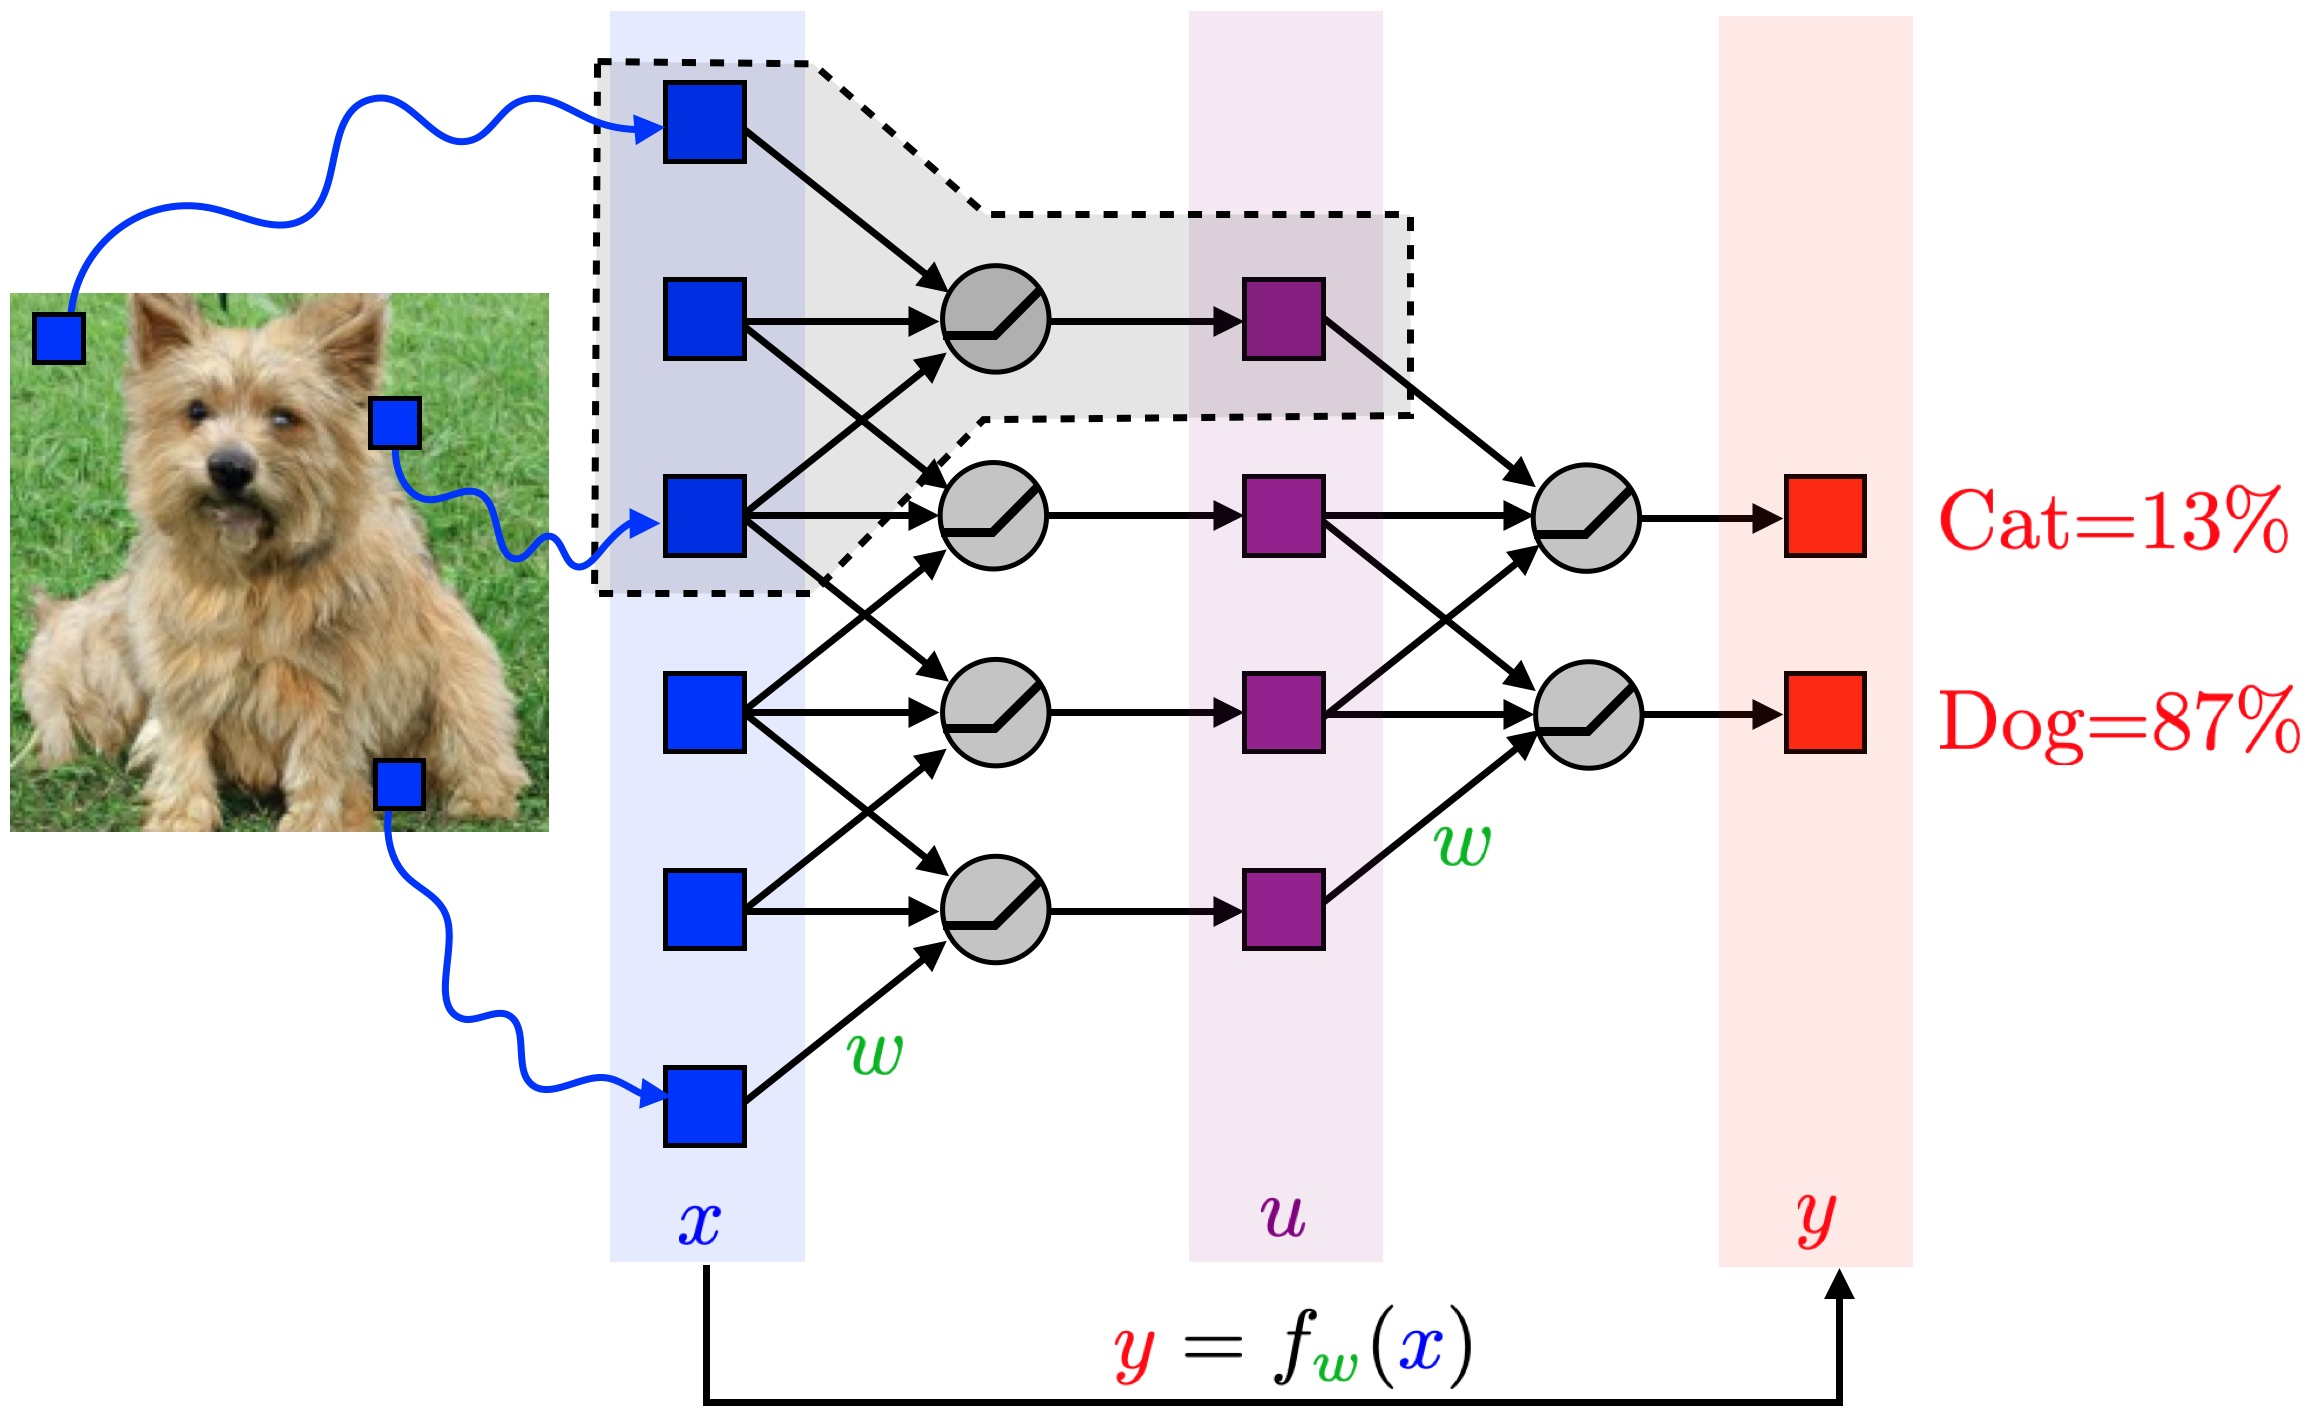
\includegraphics[width=.8\linewidth]{discriminative}
\caption{\label{fig:discriminative} 
Example of a discriminative neural network with two layers.  }
\end{figure}

Figure~\ref{fig:discriminative} details an example of such an artificial network.
%
This type of neuron was introduced in 1943 by McCulloch and Pitts~\cite{mcculloch1943logical}.
%
To simplify, it is here composed of only two layers of neurons (the first layer between ${\color{blue} x}$ and ${\color[rgb]{.5,0, .5} u}$, the second between ${\color[rgb]{.5,0,.5} u}$ and ${\color{red} y}$), but today's most efficient networks can have several dozen layers, we say that they are deeper.
%
In our example, the inputs ${\color{blue} x}$ are the pixels of an image. An image typically contains millions of pixels, and the figure voluntarily represents only a small number: a realistic network is indeed more complex. In addition, each pixel that makes up ${\color{blue} x}$ is actually made up of 3 values (one for each primary color red, green and blue).

Passing from one layer (for example the ${\color{blue} x}$ layer of inputs) to another (for example the second layer ${\color[rgb]{.5,0,.5} u}$, which is a \guill{hidden} layer in the middle of the network) is done through a set of artificial neurons. A neuron is represented on the figure~\ref{fig:neuron}. It is the first neuron, the one that calculates the first value ${\color[rgb]{.5,0,.5} u_1}$ which composes the layer ${\color[rgb]{.5,0,.5} u}$. This neuron connects a certain number of elements of the first layer (here three: ${\color{blue} x_1, x_2, x_3}$, but there can be more) to a single element of the second, so here ${\color[rgb]{.5,0,.5} u_1}$. The formula calculated by the neuron is
$$
	{\color[rgb]{.5,0,.5} u_1} = \max( \mygreen{w_1} \times \myblue{x_1} + \mygreen{w_2} \times \myblue{x_2} + \mygreen{w_3} \times \myblue{x_3} + \mygreen{w_4}, 0).
$$
The neuron thus performs a weighted sum of the three inputs, with three weights $\mygreen{w_1}, \mygreen{w_2}, \mygreen{w_3}$, and we also add $\mygreen{w_4}$, which is a bias. Then the neuron calculates the maximum between this sum and zero. One can also use a function other than the maximum function, but this one is the most popular. It is a thresholding operation. We can compare it to biological neurons which let or not pass information according to whether they are sufficiently excited or not.
%
So if the weighted sum $\mygreen{w_1} {\color{blue} x_1} + \mygreen{w_2} {\color{blue} x_2} + \mygreen{w_3} {\color{blue} x_3} + \mygreen{w_4}$ is smaller than 0, then the neuron returns the value ${\color[rgb]{.5,0,.5} u_1} = 0$, otherwise it returns the value of this sum and places it in ${\color[rgb]{.5,0,.5} u_1}$.


\begin{figure}\centering
	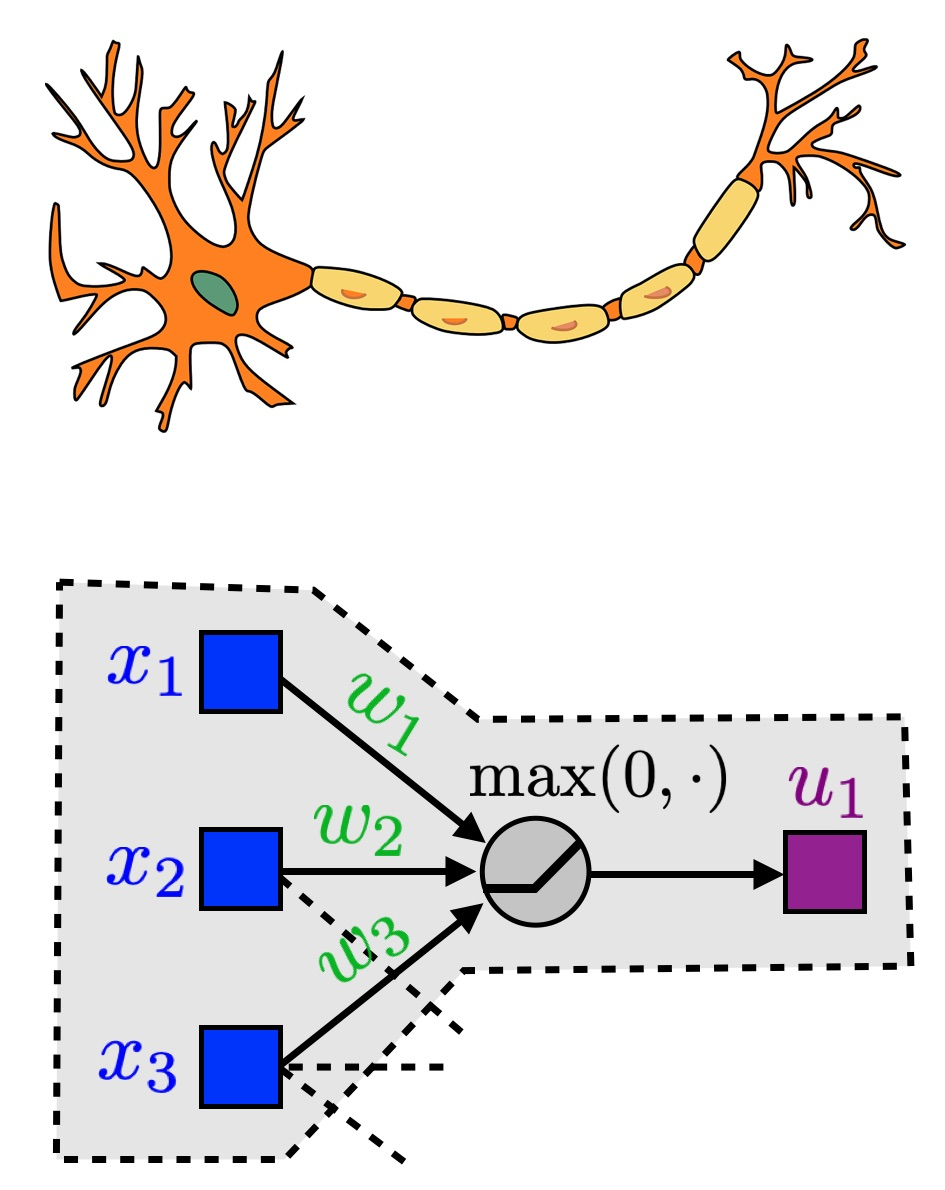
\includegraphics[width=.35\linewidth]{neuron}
\caption{\label{fig:neuron} Biological and artificial neurons. }
\end{figure}

Such neural networks were introduced by Rosenblatt~\cite{rosenblatt1957perceptron} in 1957, who called them \guill{perceptrons}. The first perceptrons contained only one layer.
%
% They were then popularized by the book by Minsky and Papert~\cite{minsky1969perceptrons}.
%
Such single-layer architectures are too simple to be able to perform complex tasks. It is by adding several layers that we can calculate more complex functions.
%
Deep neural networks thus use a very large number of layers. In recent years, these architectures have made it possible to obtain very impressive results for the recognition of images and videos as well as for the automatic translation of texts. It was this research on deep networks that enabled French researcher Yann Le Cun as well as Geoffrey Hinton and Yoshua Bengio~\cite{lecun2015deep} to obtain the Turing Prize in 2019. This prize is considered to be the equivalent of the Nobel Prize in computer science.
%
To get a better understanding of the behavior of these multi-layered networks, one can use the interactive application \url{https://playground.tensorflow.org}.

%%%%%%%%%%%%%%%%%%%%%%%%%%%%%%%%%%%%%%%%%%%%%%%%%%%%%%%%%%
\section{Supervised learning of a neural network}

Training a neural network consists in choosing the \guill{best} possible weights of the set of neurons that make up a network (for example in particular the weights $\mygreen{w_1, w_2}$ and $\mygreen{w_3}$ of the neuron shown in figure~\ref{fig:neuron}).
%
It is thus necessary to choose the values of these weights in order to best solve the task studied on a set of training data.
%
For the recognition of objects in images, this is a supervised learning problem: we have both images ${\color{blue} x}$ and the associated ${\color{red} y}$ (the probability of the presence of a cat and/or a dog in the image).
%
Figure~\ref{fig:dataset} shows some examples of images used to train a network, for which we know what they contain (the class of cats and the class of dogs).
%
It is therefore necessary, before the learning phase, that humans do a long and tedious job of labeling thousands or even millions of images.


\begin{figure}\centering
	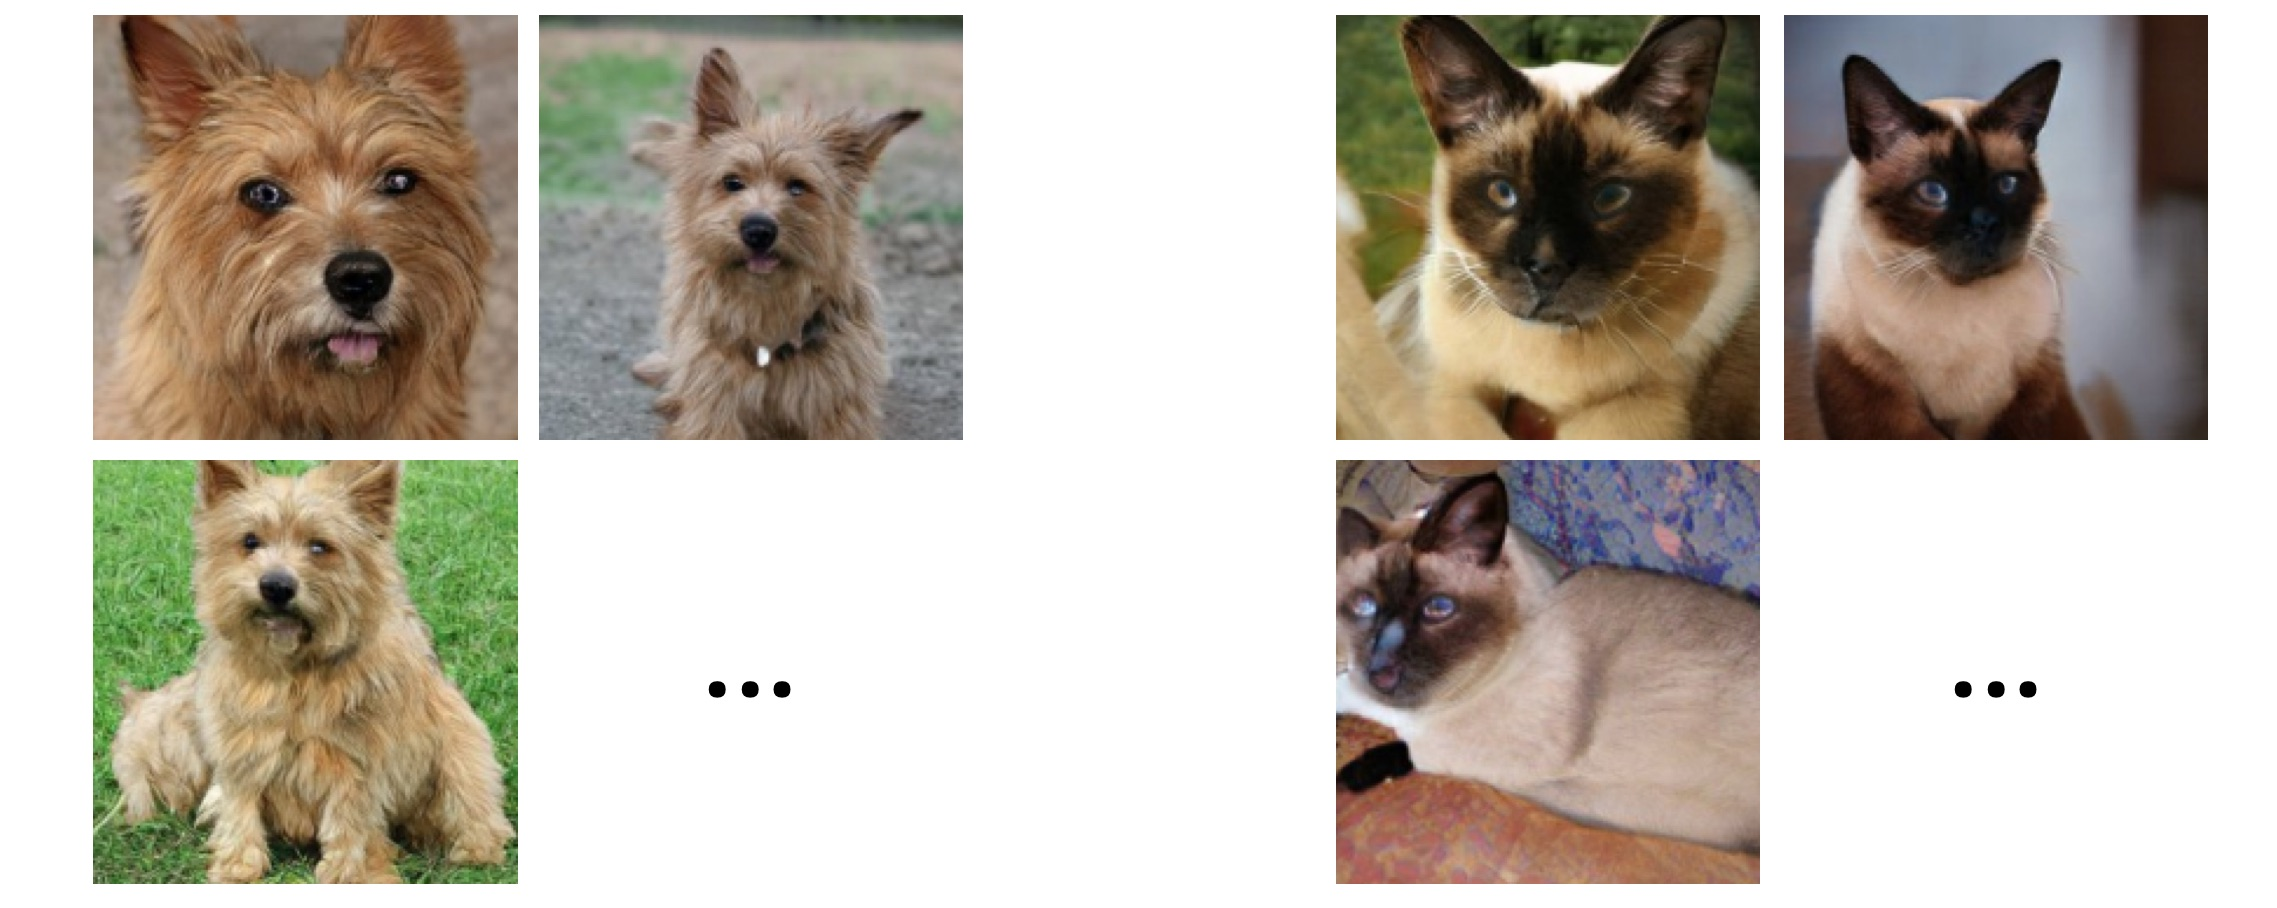
\includegraphics[width=.8\linewidth]{dataset}
\caption{\label{fig:dataset} 
Examples of images from the ImageNet database~\cite{deng2009imagenet} used for learning. }
\end{figure}

The training procedure thus consists in modifying the weights $\mygreen{w}$ such that for each ${\color{blue} x}$, the network $f_{\mygreen{w}}$ predicts as precisely as possible the ${\color{red} y}$ associated, that is to say at the end of the training that ${\color{red} y} \approx f_{\mygreen{w}}({\color{blue} x})$.
%
A simple choice is to minimize the sum $E(\mygreen{w})$ of the squares of the errors, which we write mathematically as
$$
	\min_{\mygreen{w}} E(\mygreen{w}) = \sum_{({\color{blue} x}, {\color{red} y})} (f_{\mygreen{w}}({\color{blue} x}) - {\color{red} y})^2.
$$
%
This corresponds to an optimization problem, because it is necessary to find a set of parameters which optimizes a certain quantity of interest.
%
This is a difficult problem, because there are a lot of parameters, and these parameters, especially those of the hidden layers, have a complicated influence on the result.
%
Fortunately, there are efficient mathematical and algorithmic methods to solve efficiently this type of optimization problem. They are not yet fully understood on a theoretical level and it is a very active area of research.
%
These optimization methods modify the weights $\mygreen{w}$ of the network to improve it and reduce the training error $E(\mygreen{w})$. The mathematical rule for deciding on the weight update strategy is called back propagation~\cite{rumelhart1986learning} and is a marvel of ingenuity, it is a special case of a mathematical and algorithmic method which is called backwards automatic differentiation~\cite{linnainmaa1976taylor}.

These supervised learning techniques date mainly from the 1980s. But it was only in 2012 that a paper by Krizhevsky, Sutskever and Hinton~\cite{krizhevsky2012imagenet} created a tsunami by showing that deep networks can solve complex image recognition tasks.
%
This revolution was possible thanks to the combination of three ingredients: new databases much larger than before~\cite{deng2009imagenet} ; high computing power thanks to graphical processors (\guill{GPUs}, which were previously confined to video games) ; the introduction of several optimization techniques that improve and stabilize learning~\cite{srivastava2014dropout}. 


%%%%%%%%%%%%%%%%%%%%%%%%%%%%%%%%%%%%%%%%%%%%%%%%%%%%%%%%%%
\section{The efficiency of neural networks}

George Cybenko proved in 1989~\cite{cybenko1989approximation} that a neural network$f_{\mygreen{w}}$ with two layers can approximate as precisely as one wants any continuous function $f^\star$ (so in some sense, it can  solve any task, represented by the unknown function $f^\star$, which would be able to recognize objects in any image) as long as the size of the inner layer ${\color[rgb]{.5,0,.5} u}$ (so the number of neurons) is arbitrarily large.
%
This does not mean that such a network $f_{\mygreen{w}}$ with only two layers works well in practice. To apply Cybenko's theorem, it is necessary to have a potentially infinite number of training data, which is far from being the case in practice. 
%
The ultimate goal of learning is not to minimize the learning error $E(\mygreen{w})$, but to be able to predict as precisely as possible a new data. With only a limited amount of data, one will not be able to learn precisely enough, and therefore future predictions on unseen data will be bad. The function $f_{\mygreen{w}}$ will actually be very far from the ideal function $f^\star$ that one would like to learn. 

In order to make the best possible predictions with a limited number of training data, we are therefore looking for the most suitable network architectures, which can efficiently capture the information present in the data.
%
Deep neural networks (with many layers) but with relatively few connections between layers have proven to be very effective on very \guill{structured} data such as text, sound and images.
%
For example, for an image, the pixels have neighborhood relationships, and one can impose specific connections (an architecture) and not connect a neuron with all the others but only with its neighbors (otherwise there would be too many connections). In addition, one can impose that the weights associated with a neuron are the same as those associated with another neuron. This type of networks is called convolutional networks~\cite{lecun1998gradient}.
%
For the moment, there is no mathematical analysis which explains this efficiency of deep convolutional networks. There is therefore a need for new mathematical advances to understand the behaviors and limitations of these deep networks.

